\documentclass[11pt]{article}
\usepackage[T1]{fontenc}
\usepackage[utf8]{inputenc}
\usepackage[portuguese]{babel}
\usepackage{amsmath}
\usepackage{graphicx}
\usepackage{float}
\usepackage{enumitem}

\graphicspath{{}}

\newcommand{\numpy}{{\tt numpy}}

\topmargin -.5in
\textheight 9in
\oddsidemargin -.25in
\evensidemargin -.25in
\textwidth 7in

\begin{document}

\author{Lucas Emanuel Resck Domingues}
\title{Aula prática 2
\medbreak
\large Algoritmos de resolução de sistemas lineares: \\
Algoritmos iterativos}
\maketitle

\medskip

\begin{enumerate}

\item A função Scilab foi implementada e está presente no arquivo \textit{Jacobi and Gauss-Seidel.sce} anexado.

\item Idem.

\item As funções foram testadas para o seguinte sistema linear, com vetor inicial nulo, $E = 10^{-5}$ e $M = 10000$, utilizando as três normas enunciadas:

$$\begin{cases}
    x - 4y + 2z &= 2\\
    2y + 4z &= 1\\
    6x - y - 2z &= 1
\end{cases}$$

Em nenhum dos casos a função termina com sucesso sua execução, pois o sistema não converge. Rearranjando as linhas do sistema linear de modo que a matriz dos coeficientes seja estritamente diagonal dominante e tentando novamente com vetor inicial nulo, $E = 10^{-5}$, $M = 10000$ e norma 1:

\begin{figure}[H]
    \centering
    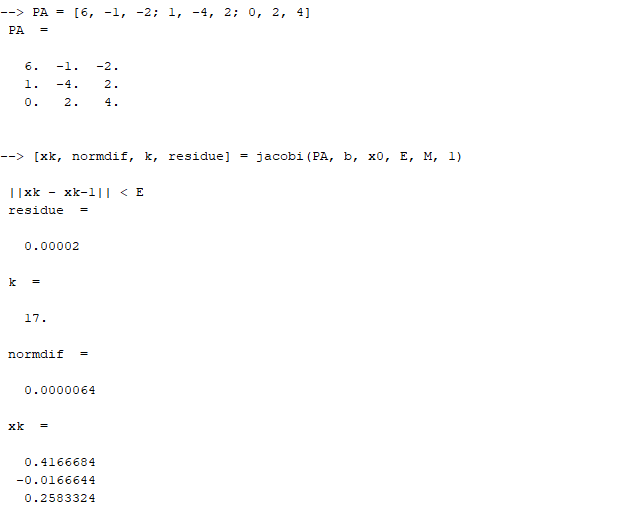
\includegraphics[]{3-Jacobi}
    \caption{Troca das linhas de $A$ e resolução com método de Jacobi.}
\end{figure}

\begin{figure}[H]
    \centering
    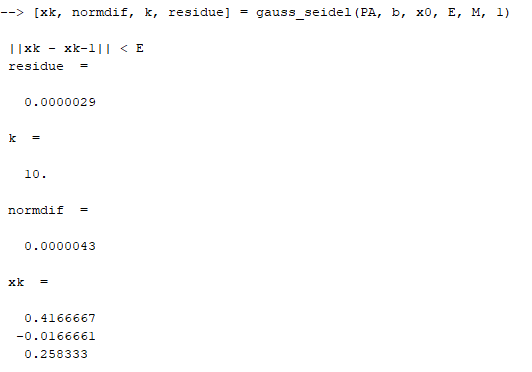
\includegraphics[]{3-Gauss-Seidel}
    \caption{Resolução com método de Gauss-Seidel.}
\end{figure}

Os dois métodos encerram o algoritmo porque $||x_k - x_{k-1}|| < E$ e retornam aproximadamente o vetor $x_k = \begin{bmatrix}
0.4166667 \\
-0.0166661 \\
0.258333 
\end{bmatrix}$.

\item

\begin{enumerate}

\item É considerado o seguinte sistema com vetor inicial nulo:

$$\begin{cases}
2x_1-x_2+x_3&=-1 \\
2x_1+2x_2+2x_3&=4 \\
-x_1-x_2+2x_3&=-5
\end{cases}$$

Utilizando $E = 10^{-5}$, M = 25 e norma 1:

\begin{figure}[H]
    \centering
    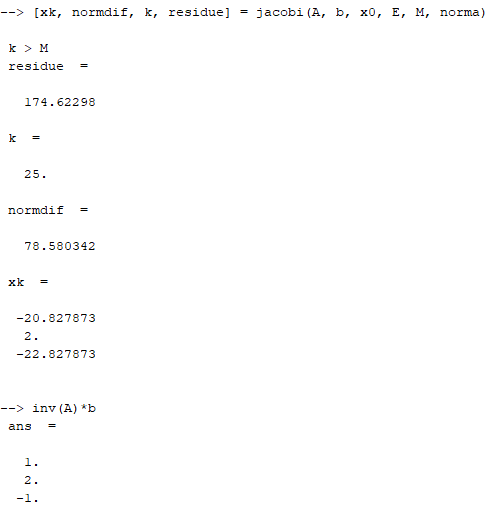
\includegraphics[]{4-a}
    \caption{O método de Jacobi falha para esse sistema.}
\end{figure}

Observe que o método de Jacobi falha em aproximar a solução para 25 iterações (compare com a solução aproximada calculada usando a inversa na Figura 3).
\bigbreak
\item Utilizando o método de Gauss-Seidel com vetor inicial nulo, $E=10^{-5}$ e norma infinito:

\begin{figure}[H]
    \centering
    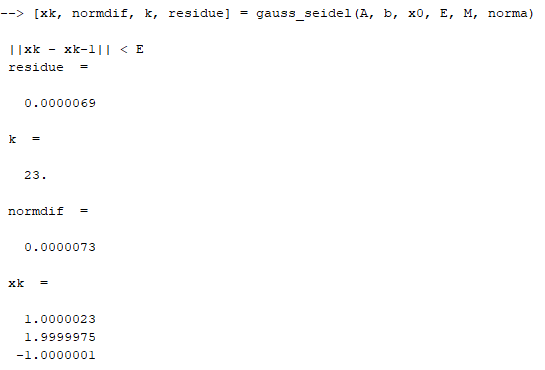
\includegraphics[]{4-b}
    \caption{Obtendo uma aproximação da solução com o método de Gauss-Seidel.}
\end{figure}

\end{enumerate}

\item

\begin{enumerate}
    \item Utilizando o método de Gauss-Seidel para o seguinte sistema linear, com $E = 10^{-2}$, $M = 300$, norma 1 e vetor inicial nulo:
    
    $$\begin{cases}
    x_1 - x_3 &= 0,2 \\
    -\dfrac{1}{2}x_1 +x_2 - \dfrac{1}{4}x_3 &= -1,425 \\
    x_1-\dfrac{1}{2}x_2+x_3 &= 2
    \end{cases}$$

    \begin{figure}[H]
    \centering
    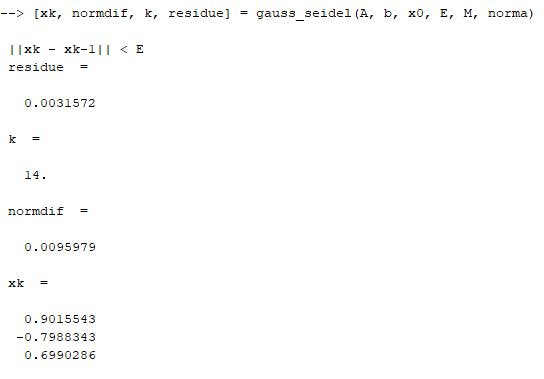
\includegraphics[]{5-a}
    \caption{Obtendo uma aproximação da solução com o método de Gauss-Seidel.}
    \end{figure}
    
    \item Alterando o sistema para 
    
    $$\begin{cases}
    x_1 - 2x_3 &= 0,2 \\
    -\dfrac{1}{2}x_1 +x_2 - \dfrac{1}{4}x_3 &= -1,425 \\
    x_1-\dfrac{1}{2}x_2+x_3 &= 2
    \end{cases}$$
    
    temos:

    \begin{figure}[H]
    \centering
    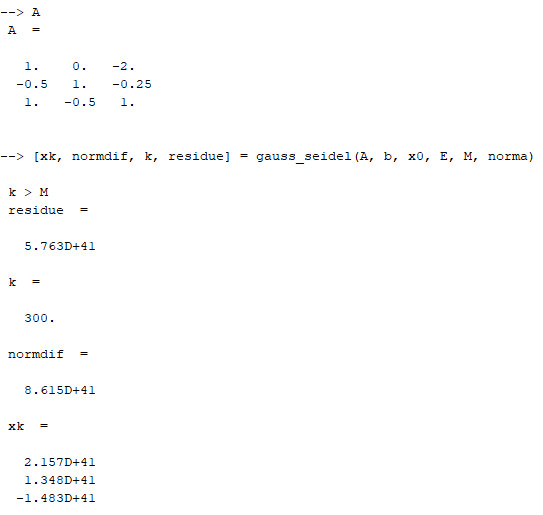
\includegraphics[]{5-b}
    \caption{O método de Gauss-Seidel falha neste caso.}
    \end{figure}
    
    Observa-se que o sistema não converge neste caso utilizando o método de Gauss-Seidel.
\end{enumerate}
    
    \item Pede-se para resolver o sistema linear composto pelas seguintes matrizes:

    \begin{figure}[H]
    \centering
    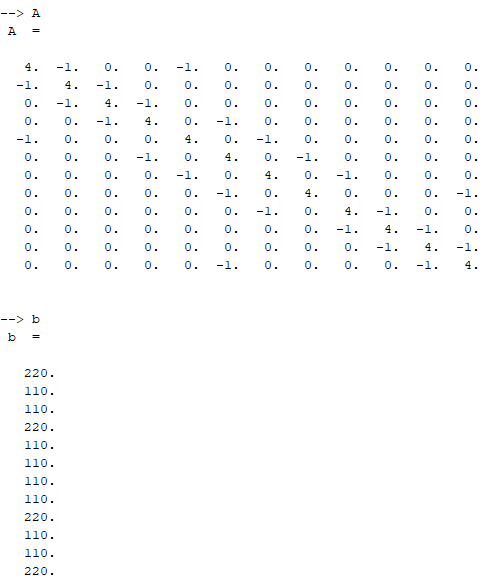
\includegraphics[]{6-b-matrices}
    \caption{Matrizes relativas ao sistema linear.}
    \end{figure}
    
    Aproximação da resolução pelo método de Jacobi com vetor inicial nulo, $E = 10^{-2}$, norma 1 e $M = 1000$:

    \begin{figure}[H]
    \centering
    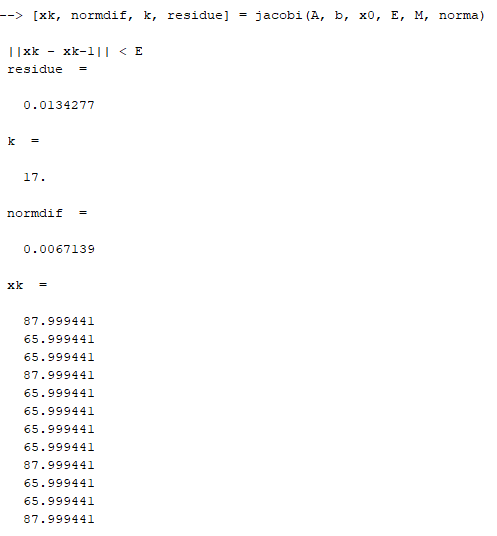
\includegraphics[]{6-b-resolution-Jacobi}
    \caption{Aproximação da resolução pelo método de Jacobi.}
    \end{figure}
    
    Aproximação da resolução pelo método de Gauss-Seidel com vetor inicial nulo, $E = 10^{-2}$, norma 1 e $M = 1000$:

    \begin{figure}[H]
    \centering
    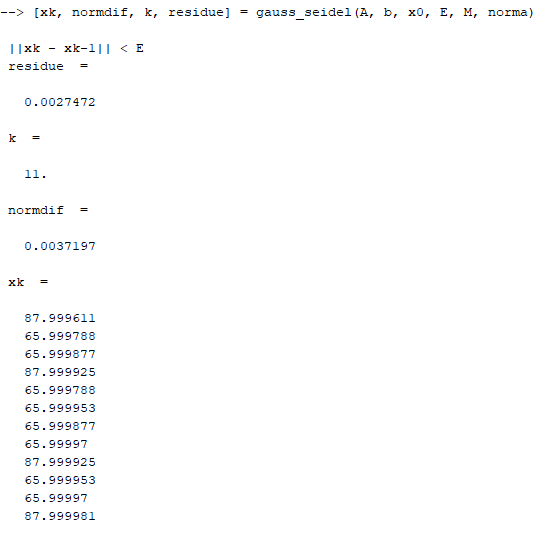
\includegraphics[]{6-b-resolution-Gauss-Seidel}
    \caption{Aproximação da resolução pelo método de Gauss-Seidel.}
    \end{figure}

\end{enumerate}

\end{document}
\grid
\grid